\newpage
\section{GoogleDirectionAPIService}
    \begin{lstlisting}[
        caption={GoogleAPIService Implementation},
        label={code:googleAPIService},
        language=java
        ]
        public class GoogleDirectionApiService implements IDirectionApi{
            //Injection the dependencies using the @Inject annotations
            // this is managed by the dagger framework checks in
            // the component 
            //which modules are to be included
            @Inject AsyncTaskUtil asyncTaskUtil;
            @Inject GoogleDirectionApiMiddleware googleDirectionApiMiddleware;
            @Inject DirectionAPI results;
            public IAsyncTaskListenerOnFinish asyncTaskListenerOnFinish;

            public GoogleDirectionApiService()  {
                asyncTaskListenerOnFinish = null;
                //This way the initialization of the dependencies 
                //are not done in this module which makes the dependencies 
                //loosely coupled
                DaggerGoogleServiceApiComponent.builder()
                        .asyncUtilModule(new AsyncUtilModule())
                        .googleServiceApiModule(new GoogleServiceApiModule())
                        .build()
                        .inject(this);

                //setting up listener which notifies (observer pattern)
                // when a response 
                //is recieved from the google API
                asyncTaskUtil.setAsyncTaskListenerOnFinish
                (new IAsyncTaskListenerOnFinish() {
                    @Override
                    public void onProcessFinish(Object result) {
                        if(asyncTaskListenerOnFinish != null) {
                            asyncTaskListenerOnFinish.onProcessFinish(result);
                            asyncTaskListenerOnFinish = null;
                        }
                        results = (DirectionAPI) result;
                    }
                });

            }

    public void getDirections(final String mode, final String origin, 
    final String destination, final String key, 
    final Map<String,String> queries) {
        //setting up a async task to run as 
        //a thread when the http request is made.
        //This ensures that the request that are being made 
        //is not blocking the code.
        asyncTaskUtil.setAsyncTaskListener(new IAsyncTaskListener() {
            @Override
            public Object asyncTaskCallback(Object... objects)  {
                DirectionAPI directions = null;
                try {
                    directions = googleDirectionApiMiddleware.
                    getWalkingDirections(mode,origin, destination, key, 
                    queries);
                } catch (IOException e) {
                    e.printStackTrace();
                }
                Log.d("Direction", directions.toString());
                return directions;
            }
        });
        asyncTaskUtil.execute();
    }

        public void setOnProcessFinish(IAsyncTaskListenerOnFinish listner) {
            asyncTaskListenerOnFinish = listner;
        }

    }
\end{lstlisting}    


\begin{figure}[htbp!]
    \centering 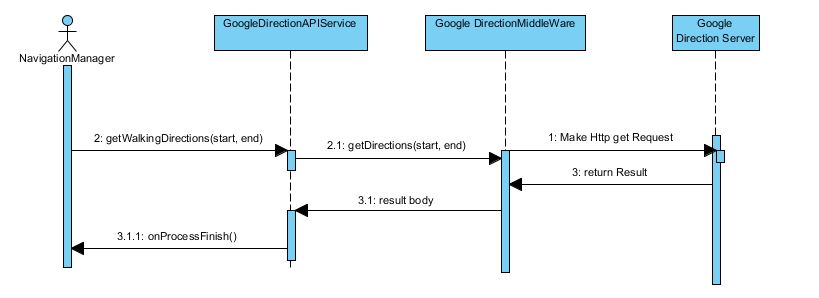
\includegraphics[scale=0.75]{grafiken/seqDigGoogleAPI.jpg}
    \caption{Sequence Diagram: Describing the functonality of the Google API service}
    \label{fig:directionServiceSeqDiagram}
\end{figure}